% !TEX root = 99_main.tex

The built environment is responsible for 19\% of global greenhouse gas emissions \cite{IPCC}. Fortunately, the use of existing technologies such as building integrated photovoltaics (BIPV), thermal insulation, and efficient building systems can mitigate up to 50\%-90\% of this emission portfolio \cite{IPCC}.\\

Thin film photovoltaics (PV) in particular have improved in terms of efficiency, cost, and light weight integration \cite{NREL, kushiya2014cis, kaelin2004low, jelle2012building}, which influenced the development of the adaptive solar facade (ASF) \cite{nagy2016adaptive}. The adaptive solar facade consists of an array of independently actuated photovoltaic panels that can move in two axes at a range of 90$^{\circ}$. An example of this technology was built at the House of Natural Resources at the ETH Zurich Campus as seen in Figure \ref{fig:introduction3}. Through the control of solar radiation, the ASF is capable of minimising the building energy consumption in terms of heating, cooling and lighting demands, while simultaneously generating electricity on site.\\

The optimum panel angles of the ASF are determined through a model control algorithm detailed in Chapter  \ref{ch:asfSimulation} \cite{jayathissa2017AE}. Simulations of building energy performance and photovoltaic electricity supply are performed for every possible combination of angles for each time step. Through an exhaustive search, the optimum combination is chosen. An ASF built on a  building with an inefficient heating system will tend to exist in a more open position in winter so that the room can heat naturally through solar radiation. Likewise, a building with an efficient heating system will tend to optimise more for the generation of electricity on site. This sensitivity to the building typology leads to an energy saving variation of 20\% - 80\% compared to an equivalent static system \cite{jayathissa2017AE, jayathissa2016PVSEC}. \\

This chapter utilises the models proposed by in Chapter  \ref{ch:asfSimulation} to extend the evaluation to a variety of building archetypes in Zurich. We will first evaluate the sensitivity of the ASF performance to the envelope resistance, and infiltration. We will then evaluate 11 building use types spanning six construction periods from the the City Energy Analyst (CEA) for ArcGIS database \cite{fonseca2016city}. By doing so, we can evaluate the optimum building properties and types for the application of an ASF. \\


The remainder of the chapter is organised as follows. The next section describes the simulation methodology. In Section \ref{ch:results3} we present the results of the case study which describes the sensitivity of the ASF to the building typology. Finally, Section \ref{ch:conclusion3} concludes the chapter.

\begin{figure}
    \centering
    \begin{subfigure}[b]{0.47\textwidth}
        \includegraphics[width=\textwidth, trim= 0cm 0cm 0cm 12cm,clip]{honr.jpg}
		\label{fig:HoNR}
    \end{subfigure} \hfill
    \begin{subfigure}[b]{0.47\textwidth}
        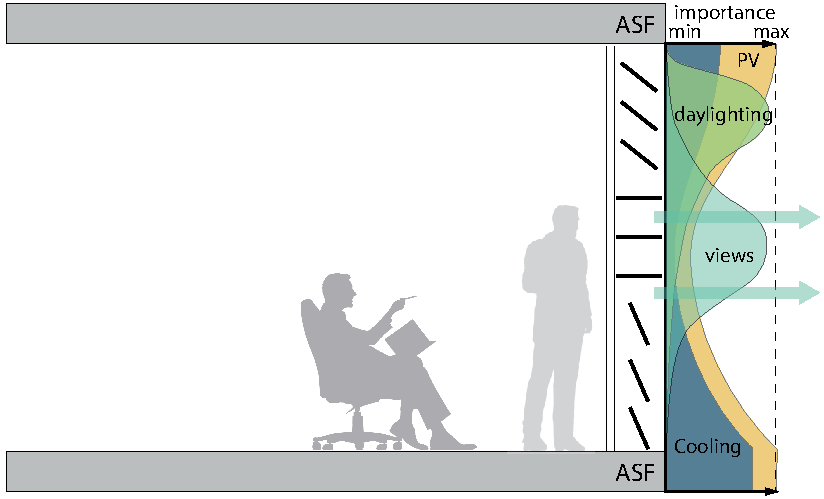
\includegraphics[width=\textwidth, trim= 0cm 0cm 0cm 0cm,clip]{facadeFunctionsnew.pdf}
		\label{fig:ASFschematic3}
    \end{subfigure}
    \caption{Left: An example of an ASF constructed at the House of Natural Resources. Right: a schematic describing how the facade can mediate solar radiation to optimise the internal environmental conditions \cite{nagy2016adaptive}}
    \label{fig:introduction3}
\end{figure}


% \begin{figure}
% \begin{center}
% \includegraphics[width=8cm, trim= 0cm 0cm 0cm 0cm,clip]{honr.jpg}
% \caption{An example of an ASF constructed at the House of Natural Resources \cite{nagy2016adaptive}}
% \label{fig:HoNR}
% \end{center}
% \end{figure}

% \begin{figure}
% \begin{center}
% 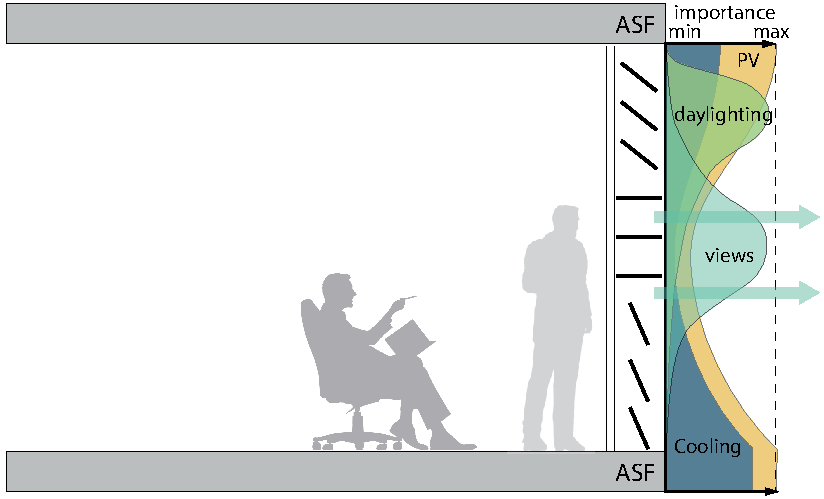
\includegraphics[width=8cm, trim= 0cm 0cm 0cm 0cm,clip]{facadeFunctionsnew.pdf}
% \caption{The facade acting as a mediator between the interior and exterior environment, while fulfilling various functions \cite{nagy2016adaptive}}
% \label{fig:ASFschematic3}
% \end{center}
% \end{figure}






